\section{Efectuarea lucrarii de laborator}



\subsection{Tasks and Points}



- Lucreaza la proiect in echipa de 2-3 persoane

- Divizeaza task-urile si descrie-le in raport, indicind pentru fiecare cine este responsabil pentru el.

- Inainte de a trece la dezvoltarea proiectului, creeaza o schema cit mai apropiata de rezultatul final (schema trebuie sa fie primul commit)

- Fiecare din membrii echipei va lucra pe propriul branch in git, iar una din persoane va avea grija sa faca merge cu master.

- Proiectul se poate afla doar in repozitoriul unui membru al echipei.

- Fiecare din membru va avea propriul raport care va include propriile observatii si concluzii.


- Basic Level (nota 5 || 6):

-

- Normal Level (nota 7 || 8):

-
 
- Advanced Level (nota 9 || 10):

- Dezvoltarea unei aplicatii:

* Desktop

* Mobile

* Web 

* Browser Extension

* Game development (web, mobile, desktop)

* Service application

* Internet application

* Client application


Incercati sa aplicati cit mai multe din thnologiile noi invatate:

* Integrarea cu baza de date

* Folosirea API

* Cross platform

* User friendly

\subsection{Analiza lucrarii de laborator}


Linkul la repozitoriu: \texttt{https://github.com/dumitritag/MIDPS-lab}


Conform celor mai noi studii, dispozitivele mobile sunt cele mai folosite device-uri din viața de zi cu zi. Incepind din anul 2016, peste 65 din cautarile de pe internet au loc de pe o tableta sau un dispozitiv mobil. Avind in vedere acest lucru, crearea unei aplicatii mobile, reprezinta un factor deosebit de important.

De aceea aplicatia aleasa de noi este una mobila. In aceasta lucrare de laborator am lucrat in echipa, eu si Dilan Nicolae. Am creat o agenda. Am utilizat IDE-ul Andoid Studio, limbajul de programare Java. Fiecare si-a avut taskurile proprii. Master in acest proiect am fost eu. Eu am creat proiectul, am implimentat pagina principala, iar Nicolae a efectuat lucrul cu baza de date.

 Android  este o platforma open source pentru dezvoltarea si rularea de aplicatii mobile. Orice aplicatie Android se bazeaza pe principiile de interactiune dintre elementele sale precum ierarhiile de layouts, containere care conduc spre copii ramurei ierarhice, widgets, simple componente UI, activities, fiecare pagina de pe layout, intents, obiecte ce reflecta legatura dintre componentele precedente. SDK-ul (Software Development Kit) Android include un set complet de instrumente de dezvoltare. Acestea includ un program de depanare, biblioteci, un emulator de dispozitiv, documentatie, mostre de cod si tutoriale. 

Pagina principa este formata dintr-un item de adaugare la meniu, ce reprezinta adaugarea unei notite. La apasarea acestuia, utilizatorul scrie notita, o salveaza sau anuleaza, dupa care are posibilitatea de a o sterge.

Am utilizat ambele metode de proiectare/definire a interfetelor utilizator: prin utilizarea de instructiuni de cod si prin definirea fisierelor descriptive XML.


  

\subsection{Imagini}




\begin{figure}[!ht]
	
	\centering
	
	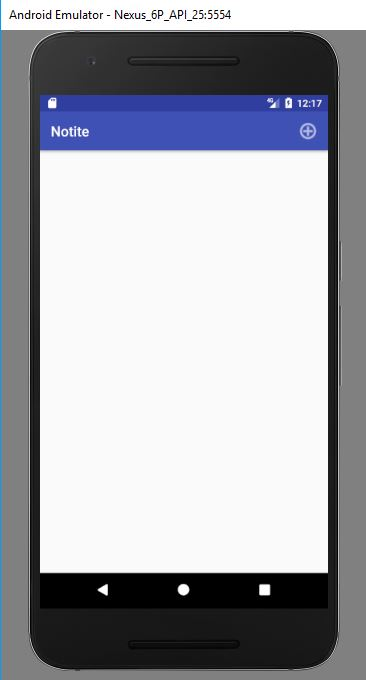
\includegraphics[width=0.5\textwidth]{Cattura.JPG}
	
	\caption{Deschiderea aplicatiei}
	
	\label{Im_label}
	
\end{figure}

\begin{figure}[!ht]
	
	\centering
	
	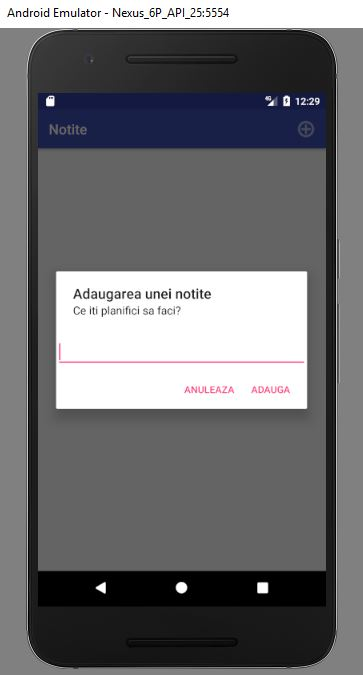
\includegraphics[width=0.5\textwidth]{Cattura1.JPG}
	
	\caption{Adaugarea notitei}
	
	\label{Im_label}
	
\end{figure}

\begin{figure}[!ht]
	
	\centering
	
	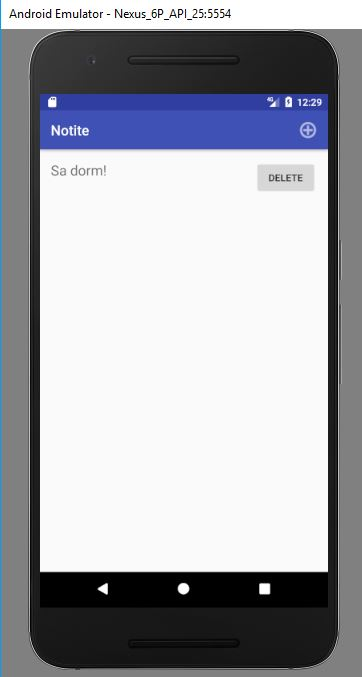
\includegraphics[width=0.5\textwidth]{Cattura2.JPG}
	
	\caption{Notita adaugata}
	
	\label{Im_label}
	
\end{figure}


\clearpage